% Copyright 2004 by Till Tantau <tantau@users.sourceforge.net>.
%
% In principle, this file can be redistributed and/or modified under
% the terms of the GNU Public License, version 2.
%
% However, this file is supposed to be a template to be modified
% for your own needs. For this reason, if you use this file as a
% template and not specifically distribute it as part of a another
% package/program, I grant the extra permission to freely copy and
% modify this file as you see fit and even to delete this copyright
% notice. 

\documentclass{beamer}

% There are many different themes available for Beamer. A comprehensive
% list with examples is given here:
% http://deic.uab.es/~iblanes/beamer_gallery/index_by_theme.html
% You can uncomment the themes below if you would like to use a different
% one:
%\usetheme{AnnArbor}
\usetheme{Antibes}%talvez
%\usetheme{Bergen}
%\usetheme{Berkeley}%talvez
%\usetheme{Berlin}
%\usetheme{Boadilla}
%\usetheme{boxes}
%\usetheme{CambridgeUS}
%\usetheme{Copenhagen}
%\usetheme{Darmstadt}
%\usetheme{default}
%\usetheme{Frankfurt}%talvez
%\usetheme{Goettingen}
%\usetheme{Hannover}
%\usetheme{Ilmenau}
%\usetheme{JuanLesPins}
%\usetheme{Luebeck}
%\usetheme{Madrid}
%\usetheme{Malmoe}
%\usetheme{Marburg}
%\usetheme{Montpellier}
%\usetheme{PaloAlto}%bomtema
%\usetheme{Pittsburgh}
%\usetheme{Rochester}
%\usetheme{Singapore}
%\usetheme{Szeged}
%\usetheme{Warsaw}

%\usepackage[brazil]{babel}
\usepackage[utf8]{inputenc}
\usepackage[brazil]{babel}
%\usepackage[latin1]{inputenc}
\usepackage{lmodern}
\usepackage{setspace}
\usepackage{verbatim}

% \usepackage{latex8}
\usepackage{subfloat}


\usepackage{algorithm}
\usepackage{algorithmic}
%\usepackage{times}
%\usepackage{amsmath}
%\usepackage{amssymb}
%\usepackage{setspace}
%\usepackage{graphicx}
%\usepackage{indentfirst}
%\usepackage{url}


\title{Aprendizado Supervisionado \\Aplicado à Predição de Links}

% A subtitle is optional and this may be deleted
%\subtitle{Optional Subtitle}

\author{Celio Henrique Nogueira Larcher Junior}
% - Give the names in the same order as the appear in the paper.
% - Use the \inst{?} command only if the authors have different
%   affiliation.

\institute[Laboratório Nacional de Computação Científica] % (optional, but mostly needed)
{
  Laboratório Nacional de Computação Científica
  %\and
  %\inst{2}%
  %Department of Theoretical Philosophy\\
  %University of Elsewhere
  }
% - Use the \inst command only if there are several affiliations.
% - Keep it simple, no one is interested in your street address.

\date{Petrópolis, 2017}
% - Either use conference name or its abbreviation.
% - Not really informative to the audience, more for people (including
%   yourself) who are reading the slides online

\subject{Ci\^encia da Computa\c{c}~ao}
% This is only inserted into the PDF information catalog. Can be left
% out. 

% If you have a file called "university-logo-filename.xxx", where xxx
% is a graphic format that can be processed by latex or pdflatex,
% resp., then you can add a logo as follows:

%\pgfdeclareimage[height=0.5cm]{university-logo}{figuras/university-logo-ufjf.png}
%\logo{\pgfuseimage{university-logo}}

% Delete this, if you do not want the table of contents to pop up at
% the beginning of each subsection:

% Let's get started
\begin{document}

\begin{frame}
  \titlepage
\end{frame}

\begin{frame}{Agenda}
\footnotesize
  \tableofcontents
  % You might wish to add the option [pausesections]
\end{frame}


\AtBeginSection[]
{
\begin{footnotesize}
  \begin{frame}<beamer>{Agenda}
    \tableofcontents[currentsection,currentsubsection]
  \end{frame}
  \end{footnotesize}
}

% Section and subsections will appear in the presentation overview
% and table of contents.


\section{O Problema de Predição de Links}



\begin{frame}{Predição de Links}
	\begin{itemize}
		\item Definição: Dado um grafo variante no tempo $G(V,E,t)$, espera-se determinar as conexões que mais provavelmente de ocorrerão em um momento futuro
		\item Este momento futuro é, em geral, delimitado por uma janela de tempo $\Delta t$
		\item Desta forma, uma outra maneira de se referir ao problema é verificar a diferença entre os grafos $G(V,E,t)$ e $G(V,E,t+\Delta t)$
	\end{itemize}
\end{frame}


\begin{frame}{Aplicações}
	\begin{itemize}
		\item Alguns exemplos de aplicações:
		\begin{itemize}
			\item Sistemas de recomendação
			\item Indicações para novas colaborações
acadêmicas
			\item Análise de possíveis conexões em redes de contado de terroristas
		\end{itemize}
	\end{itemize}
\end{frame}

\section{Aprendizado Supervisionado Aplicado à Predição de Links}

\begin{frame}{Aplicação na predição de links}
	\begin{itemize}
		\item Algoritmos de aprendizado supervisionado buscam, através de exemplos, generalizar as relações presentes nos dados
		\item O problema de predição de links se adequa de forma interessante, dado que pode ser descrito como um problema de classificação com duas classes:
		\begin{itemize}
			\item Classe 1: espera-se o surgimento de uma aresta entre o par de nós em dado intervalo de tempo
			\item Classe 2: não é previsto o surgimento de aresta entre este par de nós neste intervalo de tempo
		\end{itemize}		
		\item Os dados de entrada do sistema de aprendizado são relativos às informações de cada par de nós
	\end{itemize}
\end{frame}


\begin{frame}{Objetivo}
	\begin{itemize}
		\item Verificar quais atributos topológicos de um grafo são mais relevantes para a tarefa de predição de links via aprendizado supervisionado
		\begin{itemize}
			\item Considerar diferentes modelos de grafo (GNP, SW, PA)
			\item Verificação de diversas técnicas de aprendizado
			\item Validar os resultados em grafos obtidos de aplicações reais
		\end{itemize}
	\end{itemize}
\end{frame}


\section{Experimentos Computacionais}

\begin{frame}{Experimento}
	\begin{itemize}
		\item Experimentos realizados com auxilio do \textit{framework} Weka
		\item Mediu-se a performance da classificação de cada atributo individualmente, em um conjunto de técnicas de aprendizado
		\item As técnicas de aprendizado selecionadas foram:
		\begin{itemize}
			\item Árvore de Decisão (J48);
			\item Random Forest;
			\item Suport Vector Machine (SMO);
			\item Naive Bayes;
		\end{itemize}
		\item Como segunda etapa, mediu-se a performance da classificação no Top-5, comparado ao conjunto total de atributos
	\end{itemize}	
\end{frame}

\begin{frame}{Atributos verificados}
	\begin{itemize}
		\item \textit{short\_path}
		\item \textit{common\_neighbors}
		\item \textit{degree\_H}, \textit{degree\_L}
		\item \textit{betweenness\_centrality\_H}, \textit{betweenness\_centrality\_L}
		\item \textit{closeness\_centrality\_H}, \textit{closeness\_centrality\_L}
		\item \textit{eigenCentrality\_H}, \textit{eigenCentrality\_L}
		\item \textit{clustering\_H}, \textit{clustering\_L}
		\item \textit{eccentricity\_H}, \textit{eccentricity\_L}
	\end{itemize}
\end{frame}





\begin{frame}
	\begin{figure}[ht]
		\begin{center}
 	 	  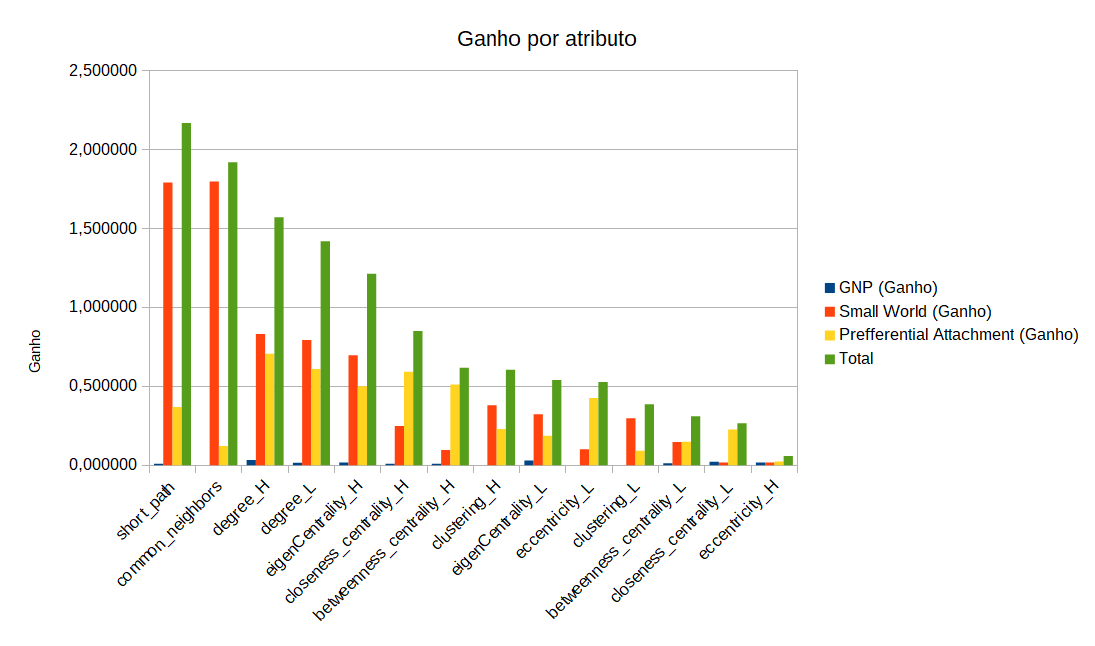
\includegraphics[scale=0.5]{figuras/attGanhoArtf.png}	
		  \label{fig:fluxogramaAG}		
%		  \caption{Tempo de processamento}	  
		\end{center}
	\end{figure}
\end{frame}

\begin{frame}{Atributos mais relevantes}
	\begin{itemize}
		\item \textit{short\_path}
		\item \textit{common\_neighbors}
		\item \textit{degree\_H}
		\item \textit{degree\_L}
		\item \textit{eigenCentrality\_H}
	\end{itemize}
\end{frame}

\begin{frame}
	\begin{figure}[ht]
		\begin{center}
 	 	  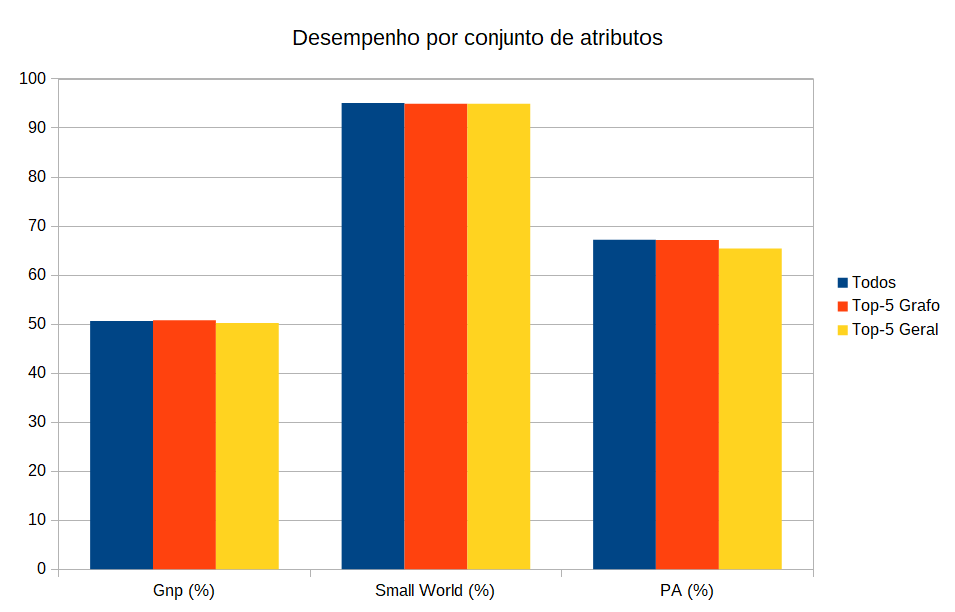
\includegraphics[scale=0.5]{figuras/attrDesempenhoArtf.png}	
		  \label{fig:fluxogramaAG}		
%		  \caption{Tempo de processamento}	  
		\end{center}
	\end{figure}
\end{frame}

%
%\begin{frame}
%	\begin{figure}[ht]
%		\begin{center}
% 	 	  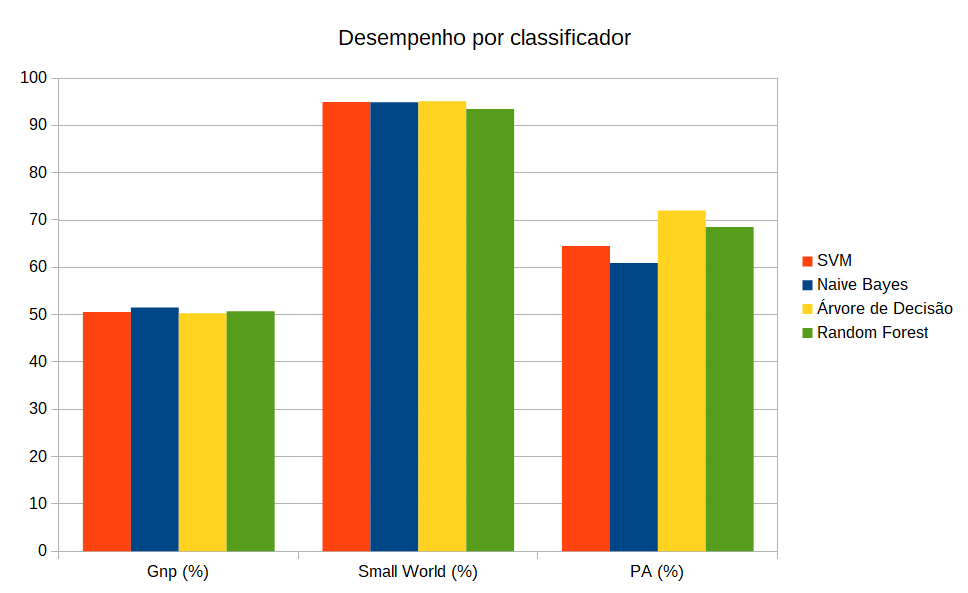
\includegraphics[scale=0.5]{figuras/classificadoresArtf.png}	
%		  \label{fig:fluxogramaAG}		
%%		  \caption{Tempo de processamento}	  
%		\end{center}
%	\end{figure}
%\end{frame}


%\begin{frame}
%	\begin{figure}[ht]
%		\begin{center}
% 	 	  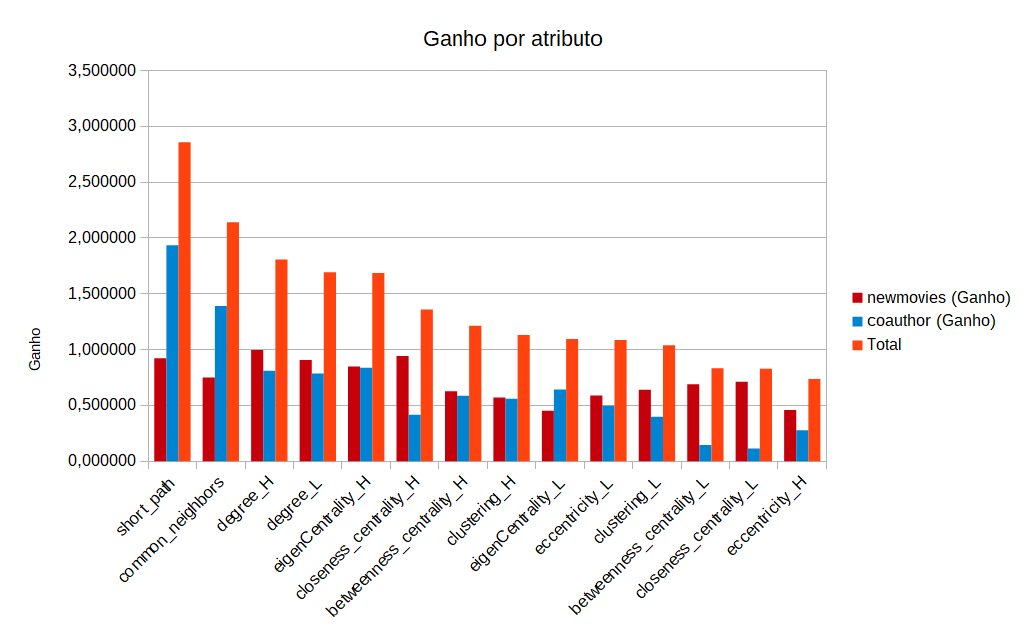
\includegraphics[scale=0.5]{figuras/attGanhoReal.png}	
%		  \label{fig:fluxogramaAG}		
%%		  \caption{Tempo de processamento}	  
%		\end{center}
%	\end{figure}
%\end{frame}



\begin{frame}
	\begin{figure}[ht]
		\begin{center}
 	 	  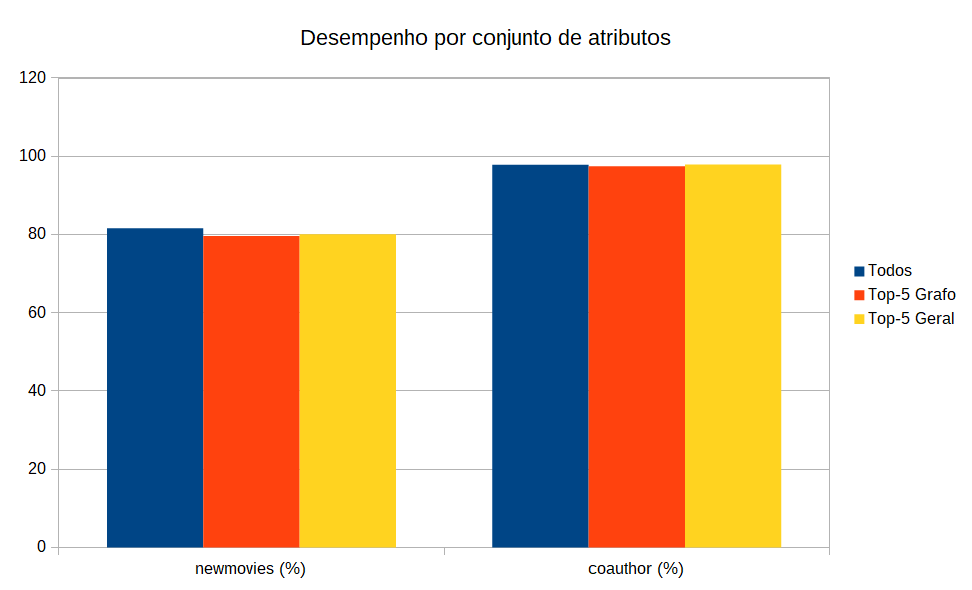
\includegraphics[scale=0.5]{figuras/attrDesempenhoReal.png}	
		  \label{fig:fluxogramaAG}		
%		  \caption{Tempo de processamento}	  
		\end{center}
	\end{figure}
\end{frame}


%\begin{frame}
%	\begin{figure}[ht]
%		\begin{center}
% 	 	  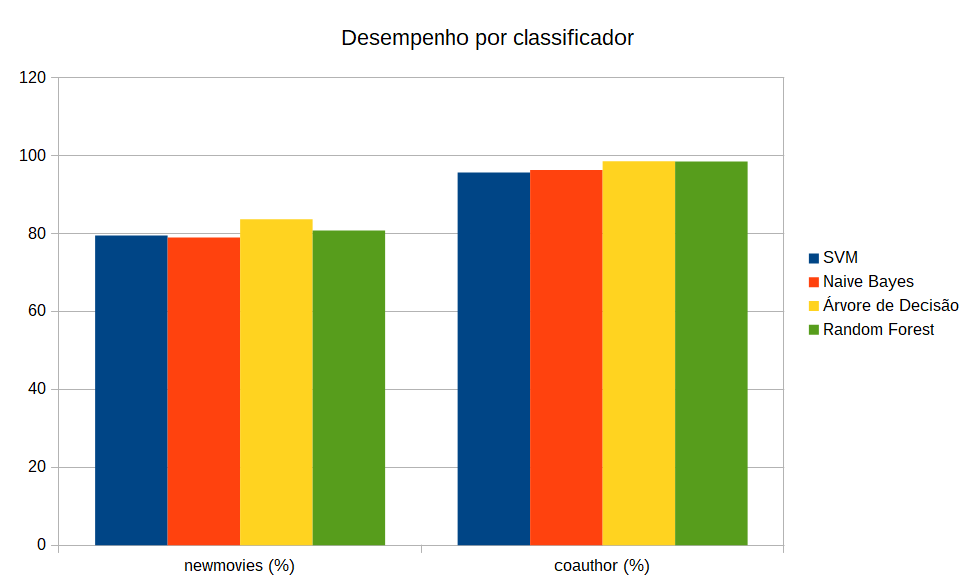
\includegraphics[scale=0.5]{figuras/classificadoresReal.png}	
%		  \label{fig:fluxogramaAG}		
%%		  \caption{Tempo de processamento}	  
%		\end{center}
%	\end{figure}
%\end{frame}



\section{Conclusões e trabalhos futuros}

\begin{frame}{Conclusões e trabalhos futuros}
	\begin{itemize}
		\item Neste trabalho foi identificado um subconjunto de atributos significativo capaz de manter a capacidade de predição 
		\item Estes atributos inclusive se apresentam na intersecção dos fatores motivadores de cada tipo de grafo analisado
		\item Outro fator, foi verificado um forte papel da política de estabelecimento das conexões na capacidade de predição
		\item Os experimento em grafos reais corroboram estas analises
		\item Como trabalhos futuros algumas possibilidades são a utilização de novas métricas e verificação dos resultados em grafos dinâmicos
	\end{itemize}
\end{frame}




\section{Refer\^encias}

% All of the following is optional and typically not needed. 
\appendix
\section<presentation>*{\appendixname}
\subsection<presentation>*{Refer\^encias}

\begin{frame}[allowframebreaks]
\scriptsize
  \frametitle<presentation>{Refer\^encias}
    
  \begin{thebibliography}{10}
  
  \beamertemplatearticlebibitems
  % Followed by interesting articles. Keep the list short.     
	
	 \bibitem{Mohammad06}
	Al Hasan, M., Chaoji, V., Salem, S., Zaki, M. (2006). 
	\newblock{Link prediction using supervised learning. \em In Proc. of SDM 06 workshop on Link Analysis, Counterterrorism and Security.}

	 \bibitem{Benchettara10}
	Benchettara, N., Kanawati, R., Rouveirol, C. (2010). 
	\newblock{Supervised machine learning applied to link prediction in bipartite social networks. \em Proceedings - 2010 International Conference on Advances in Social Network Analysis and Mining, ASONAM 2010}

	 \bibitem{Cukierski11}	
Cukierski, W., Hamner, B., Yang, B. (2011). 
\newblock{Graph-based features for supervised link prediction. \em Proceedings of the International Joint Conference on Neural Networks}

 \bibitem{Humphries08}
		Humphries M. D., Gurney K. (2008).
		\newblock{Network “Small-World-Ness”: A Quantitative Method for Determining Canonical Network Equivalence. \em Sporns O, ed. PLoS ONE}

	 \bibitem{Martinez16}
	Martinez, V., Berzal, F., Cubero, J. (2016). 
	\newblock{A Survey of Link Prediction in Complex Networks. \em ACM Computing Surveys}
	
	\bibitem{Sa11}
de Sa, H. R., Prudencio, R. B. C. (2011). 
\newblock{Supervised link prediction in weighted networks. \em In The 2011 International Joint Conference on Neural Networks}

		 \bibitem{Tang09}
		Tang, J., Sun, J., Wang, C., Yang, Z. (2009). 
		\newblock{Social Influence Analysis in Large-scale Networks. \em In Proceedings of the Fifteenth ACM SIGKDD International Conference on Knowledge Discovery and Data Mining }

	\bibitem{Wang11}
		Wang, L., Lou, T., Tang, J., Hopcroft, J. (2011). 
		\newblock{Detecting Community Kernels in Large Social Networks. \em  Proceedings of 2011 IEEE International Conference on Data Mining.}


	 \bibitem{Witten05}
		Witten, I. H., Frank, E. (2005). 
		\newblock{Data Mining: Practical Machine Learning Tools and Techniques. \em San Francisco, CA, USA: Morgan Kaufmann Publishers Inc}	
	
  \end{thebibliography}
\end{frame}

\end{document}
